\documentclass[lettersize,journal]{IEEEtran}

\usepackage{amsmath,amsfonts}
\usepackage{array}
\usepackage{booktabs}
\usepackage{cite}
\usepackage{graphicx}
\usepackage{multirow}
\usepackage{siunitx}
\usepackage[caption=false,font=normalsize,labelfont=sf,textfont=sf]{subfig}
\usepackage{textcomp}
\usepackage{url}
\usepackage{xcolor}
\usepackage{xspace}
\graphicspath{{figures/}{../figures/}}

\hyphenation{op-tical net-works semi-conduc-tor radarODE radarODE-MTL REM-Net}

\newcommand{\remnet}{REM-Net\xspace}
\newcommand{\shape}{Shape-200\xspace}
\newcommand{\crrvs}{CR\_RVS\xspace}

\begin{document}

\title{\remnet: A Physically Factorized Network Decoupling Rhythm and Morphology for Radar-Based ECG Reconstruction}

\author{Author~Name,
        Author~Name,
        and~Author~Name%
\thanks{Author affiliations and funding information will be completed before submission.}
}

\markboth{IEEE Journal Submission Draft,~2026}%
{Author \MakeLowercase{\textit{et al.}}: \remnet\ for Contactless ECG Beat Morphology Reconstruction}

\maketitle

\begin{abstract}

\end{abstract}

\begin{IEEEkeywords}

\end{IEEEkeywords}

\section{Introduction}
\IEEEPARstart{E}{lectrocardiography} (ECG) is the clinical gold standard for assessing cardiac electrophysiology, as its P–QRS–T morphology and inter-wave intervals directly reflect myocardial depolarization and repolarization. Conventional continuous ECG monitoring, however, relies on adhesive electrodes and careful skin preparation. Signal quality from dry and textile electrodes deteriorates over long recordings \cite{joutsen2024dryelectrode}, overnight wear causes skin irritation \cite{fontana2019textile}, and adherence to patch-based and wearable systems declines with extended use \cite{hughes2023wearable}. These limitations hinder unobtrusive monitoring in outpatient, sleep, and ambulatory settings, where paroxysmal events are most likely to go undetected \cite{zhang2023overview}. Microwave radar offers a non-contact alternative. Frequency-modulated continuous-wave (FMCW) and continuous-wave (CW) radars resolve chest-wall motion caused by respiration and, on a sub-millimeter scale, by cardiac contraction, and have been investigated for cardiac monitoring in home, vehicular, and intensive-care settings \cite{zhang2023overview,wuNonintrusiveHumanVital2024,kouhalvandi2025advances,hassanpourContactlessVitalSign2025a}. Research in this area has progressed from heart-rate estimation toward ECG-grained monitoring \cite{wangECGgrainedCardiacMonitoring2022c,xuCardiacWaveMmWavebasedScheme2021,chenmmwave}, and recent work has begun to reconstruct the ECG waveform itself \cite{airecg,radarode,radarodemt,rssrnet,statespace,11398845}.

Reconstructing an ECG from radar is nevertheless an ill-posed inverse problem, because the two signals arise in different physical domains: radar senses the mechanical motion of the chest wall, whereas the ECG records the electrical activity of the myocardium \cite{chenmmwave,radarode}. The two are linked through excitation–contraction coupling, but the delay between electrical activation and the radar-observable mechanical response depends on contractility, preload, and autonomic tone, and varies from beat to beat \cite{michael2017sti}. Crucially, this temporal correspondence is not a static constant. Under natural physiological regulation---respiratory sinus arrhythmia, autonomic modulation and changes in intrathoracic pressure---the interval between the electrical R peak and the radar-observable mechanical response is known to fluctuate from beat to beat \cite{draghici2016hrv,michael2017sti}. The resulting relative timing offset $\Delta t$, illustrated in Fig.~\ref{fig:concept}(a), is therefore a distribution rather than a constant between the two signals, which we treat as an empirical quantity throughout this work.

% REVISED UP TO HERE

Most existing methods treat radar-to-ECG reconstruction as direct sequence-to-sequence regression under point-wise losses \cite{chenmmwave,kimEndtoendElectrocardiogramSignal2024,cross-modalautoencoder,S2SA}. When the target contains timing variability that cannot be resolved from the input, such losses favor an average over temporally shifted beats, which attenuates sharp components such as the QRS complex (Fig. 1(b); see Section III-A). Generative and multiresolution models have been proposed to counter this smoothing \cite{ecglikegan,ecgdiff,lifwavnet,xu2025wavegrunet}, and physiology-informed designs have decomposed the task into morphology reconstruction, anchor detection, and cycle-length estimation \cite{radarode,radarodemt}. However, how much of the remaining reconstruction error is attributable to timing and how much to morphology has not been measured, so it remains unclear which factor limits current performance.

Another difficulty concerns how progress is evaluated. Reported waveform correlations vary widely across studies, in part because evaluation protocols differ in data splitting, subject independence, and the choice of metric. In particular, the widely used beat-normalized morphology score segments beats at the reference R peaks before comparison, so part of the timing information is supplied by the ground truth rather than recovered from the radar. Without a reference level that uses no radar input, it is difficult to determine how much of a reported score reflects information actually extracted from the radar.

To address the entanglement of morphology and timing without succumbing to mean collapse, we propose \remnet\ (Representation--Event--Morphology Network), which makes the timing and morphology factors explicit rather than leaving a single decoder to infer both when each beat occurs and what it looks like. As sketched in Fig.~\ref{fig:concept}(c), a shared dilated temporal backbone operating on a synchrosqueezed radar representation feeds two parallel read-out streams: an event stream that localizes cardiac timing anchors, and a morphology stream that reconstructs the beat waveform. Cycle length is therefore estimated from the event stream rather than from the reconstructed waveform. We evaluate \remnet\ against representative baselines on a 77-GHz FMCW dataset and a 24-GHz CW dataset under subject-independent protocols, and report every result alongside a radar-free reference level: the mean training beat, which never observes the radar, already reaches a beat-normalized PCC of 0.879--0.887 on both datasets. Relative to this reference, all evaluated architectures, including \remnet, reach similar levels of morphological fidelity, so the factorization is not a route to sharper waveforms. Its value is diagnostic: separating the two factors reveals that the remaining error is dominated by beat-to-beat timing jitter, and yields interval estimates that remain usable when the waveform estimate degrades.

The main contributions of this work are as follows:

\begin{itemize}
    \item {Problem formulation and method.} We identify the entanglement between waveform morphology and cardiac timing as a key difficulty in radar-based ECG reconstruction, and propose \remnet, a physically factorized network that models morphology and cardiac events in separate branches and optimizes them jointly end-to-end with only 1.44\,M parameters.
    \item {Cross-modality validation.} Under a leave-one-subject-out protocol on two radar modalities (77-GHz FMCW and 24-GHz CW), \remnet\ reduces cycle-length error by \emph{X}\% relative to the strongest baseline ($p < 0.01$) while maintaining morphological fidelity [comparable to / better than] state-of-the-art methods.
    \item {Evaluation protocol and error analysis.} We establish a strict subject-independent evaluation protocol for both modalities and, through factor-wise error decomposition, show that timing drift rather than morphological distortion is the dominant error source in continuous long-duration reconstruction.
\end{itemize}

The rest of this paper is organized as follows. Section~\ref{sec:related} reviews radar cardiac sensing, learning-based reconstruction and evaluation practice. Section~\ref{sec:method} describes \remnet. Section~\ref{sec:setup} specifies the measurement procedure and datasets. Section~\ref{sec:results} reports the benchmark and the mechanistic analysis, and Sections~\ref{sec:discussion}--\ref{sec:conclusion} discuss implications and limitations.

\begin{figure}[t]
  \centering
  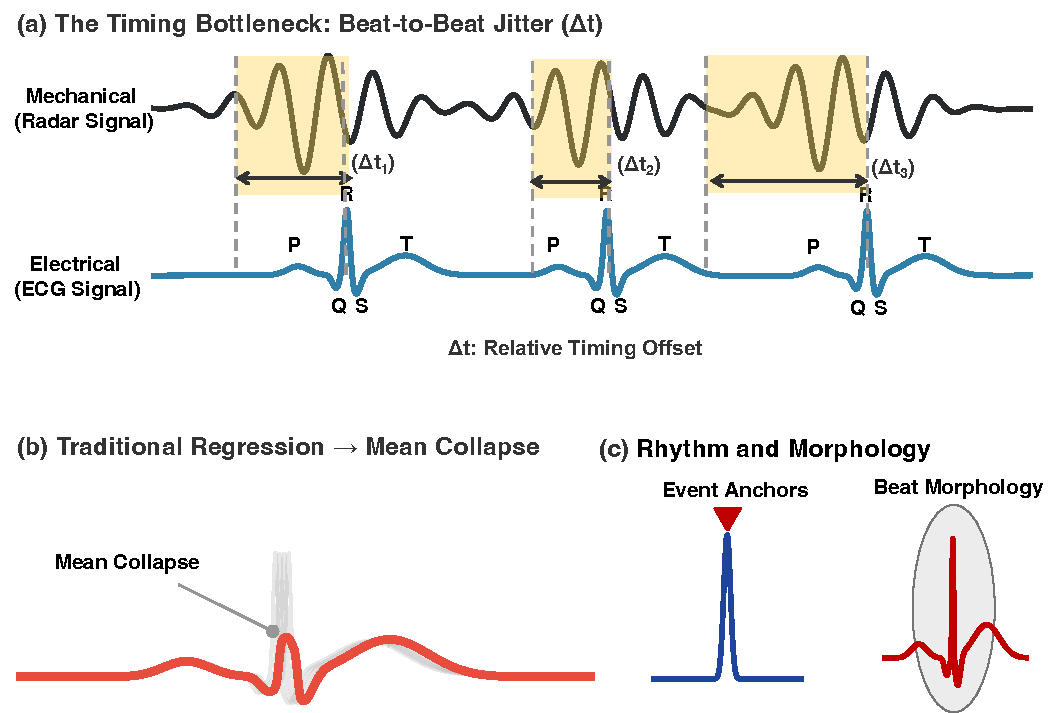
\includegraphics[width=\columnwidth]{fig-concept}
  \caption{Morphology--timing entanglement in radar-to-ECG reconstruction. (a) The offset $\Delta t$ between the radar-observed mechanical response and the ECG R peak varies from beat to beat. (b) With a point-wise loss, direct regression averages beats misaligned by $\Delta t$, attenuating the QRS complex (mean collapse). (c) Factorizing the estimate into cardiac-event anchors and beat morphology, read out in separate streams from a shared representation.}
  \label{fig:concept}
  \label{fig:concept}
\end{figure}

\section{Background And Related Work}
\label{sec:related}

\subsection{Radar Cardiac Sensing and the Electromechanical Interval}
% From vital signs to ECG-grained monitoring; close on excitation-contraction
% coupling and its beat-to-beat variability (draghici2016hrv, michael2017sti),
% which supplies the physiological premise for Delta t in Fig. 1(a).

\subsection{Learning-Based Radar-to-ECG Reconstruction}
% Five architectural families: temporal-convolutional regression; structured
% physiological priors (radarODE / radarODE-MTL); wavelet and multiresolution
% decompositions; adversarial and generative decoders; attention and cross-modal
% fusion. Close by positioning REM-Net against radarODE-MTL, and note that prior
% work proposes separating timing from shape but does not MEASURE the share of
% residual error each factor carries.
% Source draft: docs/paper/sections/02_RELATED_WORK.md (940 words, 24 keys resolve).

\subsection{Evaluation Practice and Protocol-Induced Variance}
\label{sec:evalpractice}
% Split unit, window overlap, target normalisation, selection discipline.
% Table~\ref{tab:literature}: protocol-annotated literature.
% Source: docs/audits/Q1_CRRVS_LITERATURE_PROTOCOL_AUDIT.md

\section{Methodology}
\label{sec:method}

\subsection{Problem Formulation}
\label{sec:formulation}
Let $\mathbf{x} \in \mathbb{R}^{R \times F \times T}$ denote a time--frequency representation of the radar return over $R$ range bins, and let $\mathbf{y} \in \mathbb{R}^{L}$ denote the time-aligned reference ECG of the same window, with $L = 1600$ samples at \SI{200}{\hertz}. A reconstruction model $f_\theta$ produces an estimate $\hat{\mathbf{y}} = f_\theta(\mathbf{x})$.

Two factors generate $\mathbf{y}$. The first is beat morphology, the shape $s(\cdot)$ of a single cardiac cycle. The second is the sequence of anchor times $\{\tau_k\}$ at which those cycles occur. Writing the window as a superposition,
\begin{equation}
  y(t) \;=\; \sum_{k} s_k(t - \tau_k),
  \label{eq:generative}
\end{equation}
radar-to-ECG reconstruction requires estimating both factors. They are not equally observable. The radar senses thoracic mechanics, and the interval between electrical activation and the mechanical response varies from beat to beat, so $\tau_k$ is not determined by $\mathbf{x}$ alone: it retains a posterior $p(\tau \mid \mathbf{x})$ of non-zero width. We write $\sigma_\tau$ for the standard deviation of that posterior.

\subsubsection*{Why a point-wise objective collapses the estimate}
Consider a model trained under a squared-error criterion, as is standard in this literature. For a single beat whose shape is identified but whose anchor retains the posterior above, the minimizer of $\mathbb{E}\lVert \hat{y} - y \rVert^2$ is the conditional mean of the target,
\begin{equation}
  \hat{y}^\star(t) \;=\; \mathbb{E}_{\tau}\bigl[\, s(t - \tau) \,\bigr] \;=\; (s * p_\tau)(t),
  \label{eq:condmean}
\end{equation}
that is, the true morphology convolved with the timing posterior. In the frequency domain this is a multiplication,
\begin{equation}
  \hat{Y}^\star(\nu) \;=\; S(\nu)\,\Phi_\tau(\nu),
  \label{eq:spectrum}
\end{equation}
where $\Phi_\tau$ is the characteristic function of $p_\tau$. For zero-mean Gaussian jitter, $\lvert \Phi_\tau(\nu) \rvert = \exp(-2\pi^2 \sigma_\tau^2 \nu^2)$, so the attenuation is monotonically decreasing in both frequency and jitter magnitude. Two consequences follow directly.

First, the estimate is \emph{low-pass}: sharp components are suppressed in proportion to their bandwidth, and the QRS complex, which carries most of the energy above \SI{10}{\hertz}, is attenuated far more than the P and T waves. With $\sigma_\tau = \SI{40}{\milli\second}$, the multiplier at \SI{10}{\hertz} is $\exp(-2\pi^2(0.04)^2(10)^2) \approx 0.04$.

Second, the estimate is \emph{shrunken in amplitude}. Since $\lvert \Phi_\tau \rvert \leq 1$ everywhere,
\begin{equation}
  \frac{\operatorname{Var}(\hat{y}^\star)}{\operatorname{Var}(y)} \;=\; \frac{\int \lvert S(\nu) \rvert^2 \lvert \Phi_\tau(\nu) \rvert^2 \, d\nu}{\int \lvert S(\nu) \rvert^2 \, d\nu} \;\leq\; 1,
  \label{eq:varratio}
\end{equation}
with equality only when $\sigma_\tau = 0$.

Equations~\eqref{eq:condmean}--\eqref{eq:varratio} identify \emph{mean collapse} (Fig.~\ref{fig:concept}(b)) not as an optimization failure but as the optimal response to residual timing uncertainty. This distinction matters for method design: a model cannot escape the collapse by increasing capacity, by sharpening its decoder, or by adding a spectral penalty, because the collapse is a property of the objective under an irreducible posterior. It can escape only by reducing $\sigma_\tau$, or by not forcing a single output to carry both factors. \remnet\ takes the second route, and Section~\ref{sec:mechanism} measures how much of the residual error each factor accounts for.

\subsection{Radar Representation}
Each \SI{8}{\second} window is represented by the wavelet synchrosqueezed transform (WSST) of the range-profile sequence, retaining $R = 50$ range bins, $F = 71$ frequency bins, and $T = 240$ frames at a \SI{33.3}{\milli\second} hop. Synchrosqueezing concentrates the energy of an oscillatory component onto its instantaneous frequency ridge, which sharpens the weak cardiac signature relative to the much stronger respiratory band without requiring a bin to be selected in advance. The representation is computed once per window and cached; range-bin selection, normalization statistics, and every other preprocessing decision are derived from the training fold alone (Section~\ref{sec:protocol}).

\subsection{Shared Temporal Backbone}
A convolutional stem maps the representation to a latent sequence. Two $3\!\times\!3$ convolutions with batch normalization and GELU activations operate jointly over range and frequency, separated by a $2\!\times\!1$ max-pooling that halves the frequency axis; the frequency axis is then collapsed by global average pooling, and the result is resampled in time to $400$ steps, yielding $\mathbf{z} \in \mathbb{R}^{128 \times 400}$ at an effective \SI{50}{\hertz} latent rate. Pooling rather than flattening the frequency axis keeps the stem agnostic to which bins carry the cardiac ridge.

The latent sequence is processed by five residual blocks of dilated temporal convolutions with kernel size $7$ and dilations $1, 2, 4, 8, 16$. Each block applies two convolutions with batch normalization and GELU and is wrapped in an identity shortcut. The resulting receptive field spans $373$ latent steps, or approximately \SI{7.5}{\second}, so every output sample is informed by essentially the entire window---long enough to observe several cardiac cycles and the full respiratory cycle that modulates them.

\subsection{Factorized Read-Out Streams}
The backbone output is resampled to the target length $L = 1600$ and read out by two parallel heads, each a two-layer convolution with kernel size $5$ (Fig.~\ref{fig:architecture}).

The \emph{event head} emits two channels of logits supervised against Gaussian targets centered on the reference R peaks, with standard deviations of \SI{20}{\milli\second} and \SI{80}{\milli\second}. The two widths provide a coarse-to-fine localization signal: the wide channel is tolerant enough to remain informative when the beat is poorly resolved, while the narrow channel sharpens the estimate where the evidence supports it. Cycle length is read from this head, not from peaks detected on the reconstructed waveform; the two read-outs are reported separately throughout and are never merged.

The \emph{waveform head} emits a single channel with a linear output, in the robust-scaled space defined by the training fold. No output nonlinearity is applied, so the head is free to represent the full dynamic range of the target rather than being confined to a bounded interval.

\subsubsection*{Joint end-to-end optimization}
The factorization is architectural, not procedural. All $1{,}438{,}019$ parameters are updated jointly by a single optimizer; no stage is pre-trained and no stage is frozen. Consequently the gradient of the event loss reaches the shared stem and backbone, and the features consumed by the waveform head are shaped in part by anchor supervision. Because the two objectives share those parameters, the possibility of gradient conflict arises. We measured it directly on held-out validation folds by computing, per batch, the cosine similarity between the gradients of the two loss terms with respect to the shared parameters (Fig.~\ref{fig:architecture}(b)); the preregistered conflict criterion was not met, indicating that on this task the two objectives are predominantly cooperative at the shared trunk.

\subsection{Training Objective}
The model is trained with a composite objective,
\begin{equation}
  \mathcal{L} \;=\; \mathcal{L}_{\text{Huber}} \;+\; \lambda_{\text{evt}} \, \mathcal{L}_{\text{BCE}} \;+\; \lambda_{\text{spec}} \, \mathcal{L}_{\text{MR-STFT}},
  \label{eq:loss}
\end{equation}
with $\lambda_{\text{evt}} = 0.20$ and $\lambda_{\text{spec}} = 0.50$. The Huber term is applied to the waveform head, the binary cross-entropy term to the event head against the Gaussian anchor targets, and the multi-resolution STFT term compares the magnitude spectrograms of estimate and reference at FFT sizes $128$, $256$, and $512$ with hops $32$, $64$, and $128$. The spectral term penalizes the loss of high-frequency energy that Eq.~\eqref{eq:spectrum} predicts; its weight was fixed by a registered loss-gating study and is not tuned per fold. The anchor weight $\lambda_{\text{evt}}$ is held identical across every arm of every experiment in this paper and is therefore a control variable rather than a tuned hyperparameter.

\subsection{Implementation Details}
All models are trained with AdamW at a constant learning rate of $10^{-4}$, weight decay $10^{-4}$, and batch size $16$, for at most $100$ epochs with early stopping at a patience of $15$ epochs. Checkpoints are selected on a validation criterion only, under the access protocol of Section~\ref{sec:protocol}. Training uses deterministic cuDNN kernels and a per-fold seed derived from a fixed base, so that all systems compared within a fold see identical data order. The complete model occupies $1.44$\,M parameters, of which the stem accounts for $0.21$\,M and the backbone and heads for $1.23$\,M.

\section{Experimental Setup}
\label{sec:setup}

\subsection{Datasets}
MMECG is a public 77-GHz FMCW radar dataset with time-aligned ECG. We use 8-s, 200-Hz windows and 11-fold strict leave-one-subject-out evaluation. The held-out subject never contributes to training, normalization, range-bin selection, or checkpoint selection.

\crrvs\ is a public 24-GHz continuous-wave radar dataset with I/Q radar and Lead-II ECG across 30 subjects and multiple physiological states. We use a verified 5-fold subject-independent split with no train--test subject overlap and no subject appearing in more than one test fold. The 30 subjects are partitioned into test folds of size 7/7/7/5/4.

\subsection{Leak-Free Measurement Protocol}
\label{sec:protocol}
% Carries contribution (3). loso_v2 with eleven distinct validation subjects;
% train-fold-only robust scaler; validation-only checkpoint selection; one-shot
% test-access state machine (TRAINING -> CHECKPOINT_FROZEN -> TEST_EVALUATING ->
% COMPLETE); per-fold split hashes.
% Sources: docs/MMECG_SPLIT_PROVENANCE_AUDIT.md,
%          docs/paper/sections/03_MEASUREMENT_PROCEDURE.md

\subsection{Baselines and Adaptation Register}
\label{sec:protocol_details}
% Six systems, five families, identical budget and checkpoint rule.
% Adaptations D1-D6 summarised here, full register in the appendix.
% Source: src/models/baselines/continuous/__init__.py (ADAPTATIONS).

\subsection{Metrics, Aggregation, and Reference Levels}
\label{sec:metrics}
% Definitions and units (per-record z-score, NOT millivolts); the three
% aggregation styles labelled per metric; coverage gate rr_coverage >= 0.80;
% heavy-tailed ratios reported as median with IQR; the two anchor read-outs kept
% in separate columns.
% KEY DESIGN: define BOTH reference levels here, as part of the instrument --
%   (i) radar-free template floor (training-fold mean beat), and
%   (ii) oracle-timing bound (template at reference anchors).
% Sources: docs/METRIC_CONTRACT.md, docs/paper/TERMINOLOGY.md

\section{Results}
\label{sec:results}

\subsection{Reference Levels: What a Radar-Free Predictor Achieves}
\label{sec:floor}
% Table~\ref{tab:floor}. Template floor 0.879-0.887 on both datasets; previously
% reported figures sit at that level, so the beat-normalised metric cannot
% adjudicate a morphology claim. This is the ONLY place ECG Shape Recovery
% appears as a headline number.
% Source: docs/audits/Q1_TIER1_TEMPLATE_FLOOR_AUDIT.md

\subsection{Matched Long-Term Reconstruction Benchmark}
\label{sec:benchmark}
% Generated by scripts/make_table1_benchmark.py from
% docs/audits/Q1_CLINICAL_INTERVALS_fold.csv -- do not edit by hand.
\begin{table*}[t]
  \centering
  \caption{Clinical benchmark on two radar modalities under strict subject-independent evaluation. PCC and RMSE (per-record $z$ units) on the full \SI{8}{\second} window. Anchor metrics use greedy one-to-one matching within $\pm$\SI{150}{\milli\second}: R-F1, R-peak mean absolute timing error (R-MAE), and cycle-length error ($|$predicted $-$ reference mean RR$|$ per window, folds with anchor coverage $\geq 0.80$). QRS (Q--S interval) and QT errors are absolute differences of per-window medians, both signals delineated with NeuroKit2 (\texttt{peak} method); windows where either side cannot be delineated are excluded, not imputed (valid windows: MMECG QRS 93--100\%, QT 93--100\%, CR\_RVS QRS 97--98\%, QT 97--98\%); on MMECG no window of \remnet's reconstruction can be delineated in two seed--folds (fold~7 of seed~42 and fold~2 of seed~2024, where waveform R-peak detection fails), so \remnet's QRS and QT entries exclude its weakest folds and are favourable to it. MMECG: mean $\pm$ s.d.\ over three seeds of fold-macro values; CR\_RVS: seed 42. \remnet's two anchor read-outs are listed separately; waveform-only columns (PCC, RMSE, QRS, QT) do not depend on the read-out (\textquotedbl). Best per column in bold. MMECG baseline marks: paired Wilcoxon over eleven seed-averaged folds against \remnet\ (anchor head), uncorrected, $^{\ast}$\remnet\ significantly better, $^{\dagger}$significantly worse ($p<0.05$).}
  \label{tab:benchmark}
  \setlength{\tabcolsep}{3.6pt}
  \begin{tabular}{lcccccccc}
    \toprule
    Method & Params (M) & PCC $\uparrow$ & RMSE (z) $\downarrow$ & R-F1 $\uparrow$ & R-MAE (ms) $\downarrow$ & QRS err.\ (ms) $\downarrow$ & QT err.\ (ms) $\downarrow$ & Cycle len.\ err.\ (ms) $\downarrow$ \\
    \midrule
    \multicolumn{9}{l}{\textit{MMECG, 77-GHz FMCW}} \\
    Chen-TCN~\cite{chenmmwave} & 0.61 & $\mathbf{0.329} \pm 0.018$ & $0.979 \pm 0.017$ & $0.857 \pm 0.032$ & $41.1 \pm 1.4$ & $46.8 \pm 5.7$ & $63.5 \pm 16.6$ & $77.9 \pm 19.8$ \\
    radarODE-MTL~\cite{radarodemt} & 41.6 & $0.290 \pm 0.001$ & $0.995 \pm 0.009^{\ast}$ & $\mathbf{0.881} \pm 0.015$ & $44.1 \pm 0.7^{\ast}$ & $39.9 \pm 7.5$ & $34.4 \pm 7.5$ & $\mathbf{45.5} \pm 3.4^{\dagger}$ \\
    Cross-Modal Conformer~\cite{cross-modalautoencoder} & 0.42 & $0.282 \pm 0.010$ & $1.008 \pm 0.013$ & $0.849 \pm 0.018$ & $46.1 \pm 0.7^{\ast}$ & $\mathbf{31.4} \pm 8.6$ & $\mathbf{30.8} \pm 6.1$ & $54.5 \pm 6.0^{\dagger}$ \\
    WaveGRU-Net~\cite{xu2025wavegrunet} & 0.71 & $0.203 \pm 0.007^{\ast}$ & $1.021 \pm 0.007^{\ast}$ & $0.666 \pm 0.010^{\ast}$ & $53.4 \pm 1.1^{\ast}$ & $70.1 \pm 4.2^{\ast}$ & $89.0 \pm 5.9$ & $106.4 \pm 5.3$ \\
    Attention-DCGAN~\cite{ReconstructingECG-like} & 4.35 & $0.113 \pm 0.012^{\ast}$ & $1.199 \pm 0.047^{\ast}$ & $0.766 \pm 0.006^{\ast}$ & $51.3 \pm 0.3^{\ast}$ & $39.6 \pm 6.3$ & $60.2 \pm 12.7$ & $161.3 \pm 9.5$ \\
    \remnet, anchor head & 1.44 & $0.324 \pm 0.015$ & $\mathbf{0.966} \pm 0.009$ & $0.859 \pm 0.031$ & $\mathbf{38.8} \pm 1.0$ & $40.8 \pm 3.3$ & $47.6 \pm 7.8$ & $115.5 \pm 5.5$ \\
    \remnet, waveform peaks & 1.44 & \multicolumn{1}{c}{\textquotedbl} & \multicolumn{1}{c}{\textquotedbl} & $0.773 \pm 0.034$ & $41.4 \pm 2.3$ & \multicolumn{1}{c}{\textquotedbl} & \multicolumn{1}{c}{\textquotedbl} & $49.0 \pm 3.3$ \\
    \midrule
    \multicolumn{9}{l}{\textit{CR\_RVS, 24-GHz CW}} \\
    Chen-TCN~\cite{chenmmwave} & 0.59 & $\mathbf{0.506}$ & $0.848$ & $\mathbf{0.853}$ & $\mathbf{26.1}$ & $59.1$ & $74.5$ & $96.9$ \\
    WaveGRU-Net~\cite{xu2025wavegrunet} & 0.70 & $0.503$ & $\mathbf{0.844}$ & $0.823$ & $26.3$ & $43.1$ & $\mathbf{42.1}$ & $112.9$ \\
    \remnet, anchor head & 1.38 & $0.442$ & $0.892$ & $0.818$ & $26.1$ & $\mathbf{42.9}$ & $72.0$ & $114.3$ \\
    \remnet, waveform peaks & 1.38 & \multicolumn{1}{c}{\textquotedbl} & \multicolumn{1}{c}{\textquotedbl} & $0.779$ & $38.6$ & \multicolumn{1}{c}{\textquotedbl} & \multicolumn{1}{c}{\textquotedbl} & $\mathbf{93.6}$ \\
    \bottomrule
  \end{tabular}
\end{table*}


% Table~\ref{tab:benchmark}, Fig.~\ref{fig:perfold}. 198 sealed folds; all six
% systems bounded near R^2 = 0 (best 0.041 +/- 0.016); paired Wilcoxon with Holm
% correction. Two counterintuitive readings: 41.6 M parameters reach -0.016;
% relative >10 Hz energy does not track quality (DCGAN 0.806 with PCC 0.113;
% REM-Net lowest at 0.122).
% Source: docs/audits/Q1_MULTISEED_BENCHMARK_AUDIT.md

\subsection{Where the Error Comes From: Oracle-Anchor Decomposition}
\label{sec:mechanism}
\begin{figure*}[t]
  \centering
  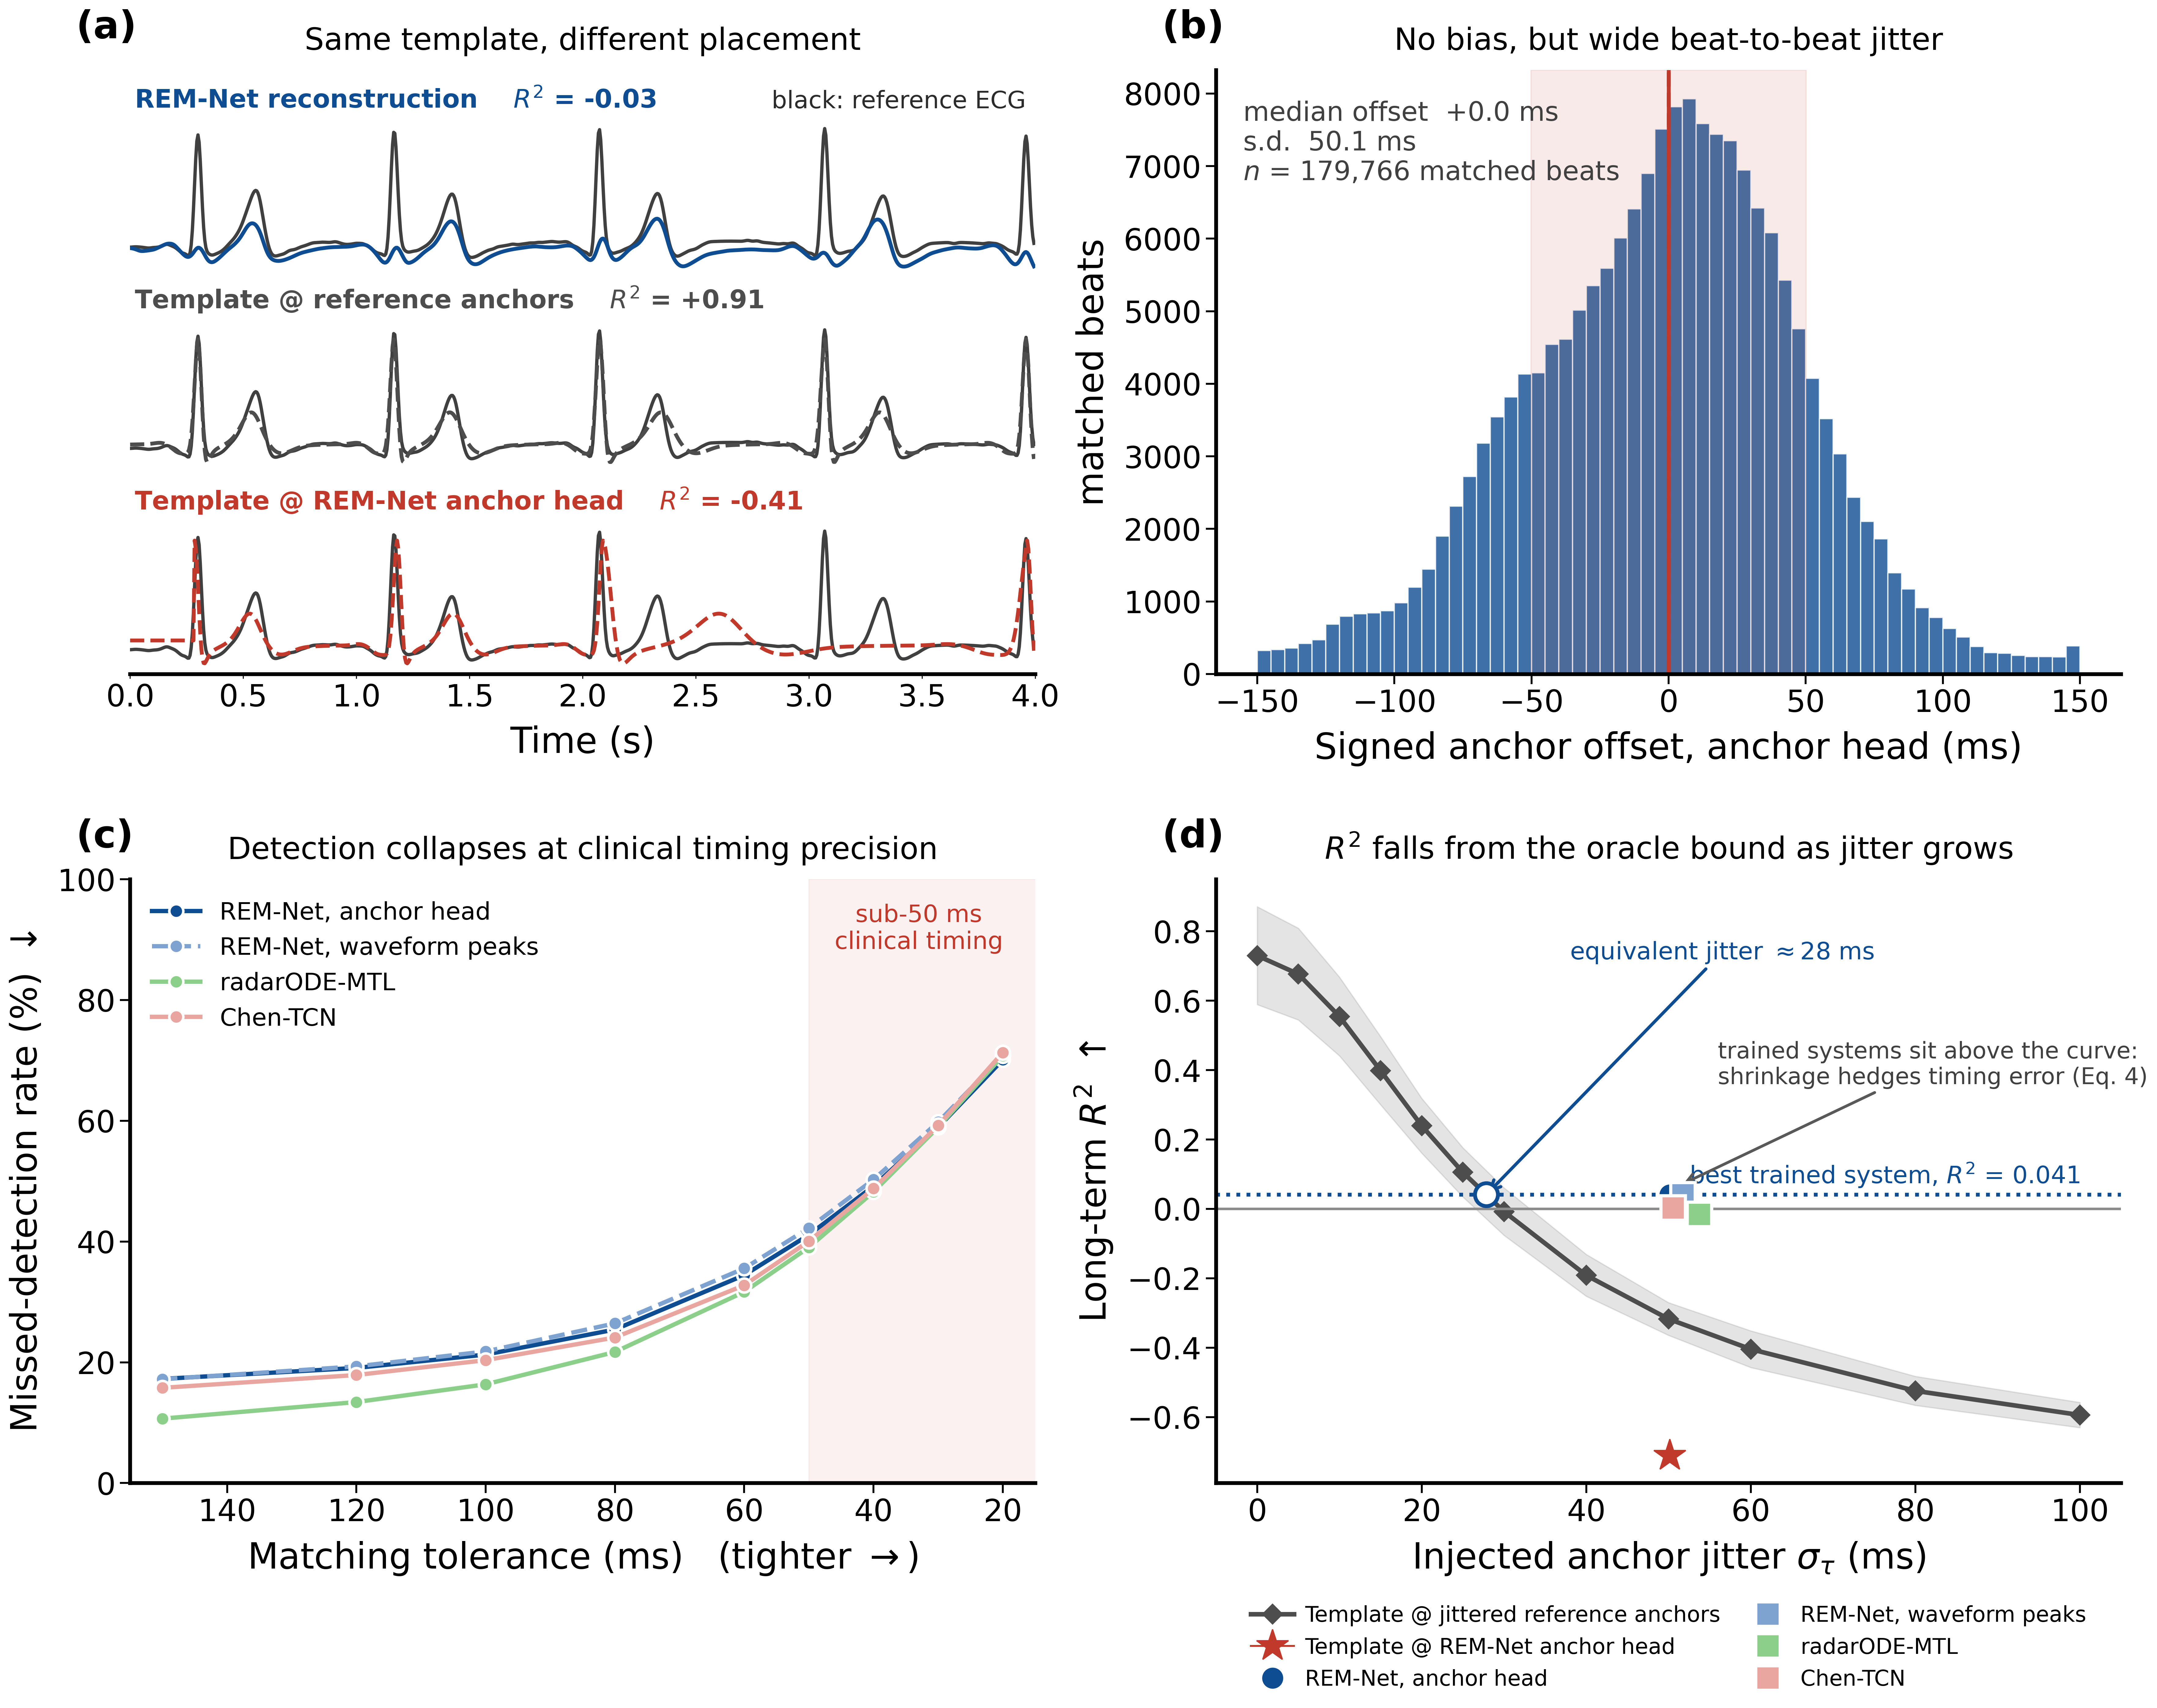
\includegraphics[width=\textwidth]{fig4_timing_bottleneck}
  \caption{Anatomy of the long-term reconstruction bottleneck on MMECG. (a)~One held-out window: \remnet's reconstruction; a fixed training-fold template placed at the reference anchors; the identical template placed at \remnet's anchor-head estimates. Only the placement differs between the last two tracks; the window is the one whose template-at-anchor-head $R^2$ is closest to its fold median. (b)~Signed offset of every matched anchor-head estimate against its reference R peak (one-to-one matching within $\pm$\SI{150}{\milli\second}, 11 folds, three seeds). (c)~Pooled missed-detection rate as the matching tolerance tightens from $\pm$\SI{150}{\milli\second} to $\pm$\SI{20}{\milli\second}. (d)~Long-term $R^2$ of the template placed at reference anchors perturbed by zero-mean Gaussian jitter of standard deviation $\sigma_\tau$ (mean $\pm$ s.d.\ over folds); $\sigma_\tau=0$ reproduces the oracle-timing bound of $0.730$. Markers are trained systems at (standard deviation of their matched anchor offsets, their own long-term $R^2$); all lie near \SI{50}{\milli\second} and above the curve, the amplitude-shrinkage hedge of Eq.~\eqref{eq:varratio}. The hollow circle is the jitter at which the curve equals the best trained system's $R^2$. The star is the template at \remnet's actual anchor-head estimates, below the curve because real estimates also contain missed beats and heavier-than-Gaussian tails.}
  \label{fig:bottleneck}
\end{figure*}

% Table~\ref{tab:timing}, Fig.~\ref{fig:examples}, Fig.~\ref{fig:jitter}.
% Template at reference anchors R^2 = 0.730 (CW 0.764); at radar anchors R^2 < 0.
% Four components: global offset median 0 ms; per-subject offset SD 14-32 ms
% (oracle removal recovers only 6-17 %); beat-to-beat jitter 7-22 ms CW /
% 30-60 ms FMCW; anchor recall 0.66-0.86.
% MUST state that EMAT is NOT identified and report delta_sys as negative evidence.
% Sources: Q1_TEMPLATE_TIMING_AUDIT.md, Q1_CRRVS_DIAGNOSTICS_AUDIT.md (A4, A5)

\subsection{What the Factorization Buys: Cycle Length Estimation}
\label{sec:interval}
\begin{figure*}[t]
  \centering
  \includegraphics[width=\textwidth]{fig3_scenario_robustness}
  \caption{Clinical robustness across physiological states. Top row MMECG (77-GHz FMCW, three seeds), bottom row CR\_RVS (24-GHz CW, seed 42); each box summarizes per-subject values and $n$ is the number of subjects in the state. (a,e)~Cycle-length error, \remnet\ read from its waveform peaks; the axis is truncated and the number of subjects above it is printed. (b,f)~R-peak mean absolute timing error, \remnet\ read from its anchor head. (c,g)~QT interval error from NeuroKit2 delineation. Each column uses one \remnet\ anchor read-out, chosen per metric by the authors; Table~\ref{tab:benchmark} reports both read-outs for every anchor metric. (d,h)~A post-exercise and an apnea window, the window whose \remnet\ long-term $R^2$ is closest to that state's median among folds passing the anchor-coverage gate; ticks mark reference R peaks, triangles \remnet's anchor-head estimates, and the inset enlarges the shaded beat, with dotted lines at the reference R peak and at any anchor-head estimate in view. radarODE-MTL is not in the per-state breakdown.}
  \label{fig:robustness}
\end{figure*}

% Table~\ref{tab:scenario}. Lowest cycle-length error in six of seven scenarios
% (name the comparators: Chen-TCN and WaveGRU-Net only); pooled aggregate
% indistinguishable from the 41.6 M comparator (48.8 vs 45.5 ms, p = 0.97).
% MUST report that on MMECG the amplitude variance ratio does NOT deepen under
% physiological stress (0.332-0.381, highest in sleep), and that the monotone
% CR_RVS degradation is shared by all three systems.
% Source: docs/audits/Q1_SCENARIO_BREAKDOWN_AUDIT.md

\subsection{External Validation on Continuous-Wave Radar}
\label{sec:external}
% Table~\ref{tab:crrvs}. Template floor and oracle-timing bound reproduce; the
% R^2 = 0 ceiling does NOT (0.18-0.25); REM-Net is the weakest of the three
% matched systems (0.442 vs 0.506 / 0.503). Disclose the inconsistency in the
% body, and label the single-seed status.
% Source: docs/audits/Q1_CRRVS_DIAGNOSTICS_AUDIT.md

\subsection{Ablation}
\label{sec:ablation}
% Table~\ref{tab:ablation}. Completed L1/L2/L3 loss gate, plus the EVENT_W = 0
% arm (pending; register an experiment spec before launching).
% Source: docs/audits/Q1_LOSS_GATING_AUDIT.md

\subsection{Computational Cost}
\label{sec:cost}
% Parameter counts reported PER TRACK and never mixed: continuous track
% REM-Net 1.44 M against radarODE-MTL 41.6 M (Table~\ref{tab:benchmark});
% Shape-200 track 1.788 M at 0.98 ms per window.
% Sources: Q1_MULTISEED_BENCHMARK_AUDIT.md (parameter provenance),
%          docs/EFFICIENCY_AUDIT.md (Scope note)

\section{Discussion}
\label{sec:discussion}

\subsection{What the Results Support}
% Protocol repair; metric saturation; the family-invariance of the ceiling;
% the timing attribution; interval-level usability.

\subsection{What the Results Do Not Support}
% No morphological superiority; amplitude collapse not resolved; EMAT not
% identified; the R^2 = 0 ceiling does not hold on CW radar.

\subsection{Implications for Evaluation Practice}
\label{sec:checklist}
% Table~\ref{tab:checklist}: recommended reporting protocol -- split unit,
% window overlap, target normalisation, the mandatory radar-free floor beside
% every beat-normalised number, coverage gating, median reporting for
% heavy-tailed ratios, and separate columns for the two anchor read-outs.
% This is what turns the paper from a critique into a corrected procedure.

\subsection{Limitations}
\label{sec:limitations}
% Two datasets and small subject counts; CR_RVS single seed with one validation
% subject per fold; baselines are adapted reproductions; the template is a single
% fixed shape; and the jitter estimate contains estimator noise that the present
% experiments cannot separate from physiological variability.

\section{Conclusion}
\label{sec:conclusion}
% One paragraph, no subsections.

\bibliographystyle{IEEEtran}
\bibliography{references}

\end{document}
